%-------------------------------------------------------------------------------

% This file is part of Code_Saturne, a general-purpose CFD tool.
%
% Copyright (C) 1998-2011 EDF S.A.
%
% This program is free software; you can redistribute it and/or modify it under
% the terms of the GNU General Public License as published by the Free Software
% Foundation; either version 2 of the License, or (at your option) any later
% version.
%
% This program is distributed in the hope that it will be useful, but WITHOUT
% ANY WARRANTY; without even the implied warranty of MERCHANTABILITY or FITNESS
% FOR A PARTICULAR PURPOSE.  See the GNU General Public License for more
% details.
%
% You should have received a copy of the GNU General Public License along with
% this program; if not, write to the Free Software Foundation, Inc., 51 Franklin
% Street, Fifth Floor, Boston, MA 02110-1301, USA.

%-------------------------------------------------------------------------------

\newpage
%-------------------------------------------------------------
\section{CASE 4: Head loss, parallelism and spatial average}
%-------------------------------------------------------------
\label{prg_case4}%
This case will be run in parallel on two processors. Head loss will be used to
simulate the presence of an obstacle in the flow and the spatial average of the
temperature will be calculated at each time step.

        \subsection{Calculation options}
%-----------------------------------------

The options for this case are the same as in case 3:
\begin{itemize}
\renewcommand{\labelitemi}{$\rightarrow$}
        \item Flow type: unsteady flow
        \item Time step: uniform and constant
        \item Turbulence model: $k-\epsilon$
        \item Scalar(s): 1 - temperature\\
      \hspace*{1.6cm} 2 - passive scalar
        \item Physical properties: uniform and constant (except density)
        \item Management of monitoring points
\end{itemize}


        \subsection{Initial and boundary conditions}
%---------------------------------------------------

\begin{itemize}
\renewcommand{\labelitemi}{$\rightarrow$}
        \item Initialization: 20\degresC\ for temperature (default value) \\
        \hspace*{2.1cm}        10 for the passive scalar
\end{itemize}

The boundary conditions are defined in the user interface and depend on the
boundary zone.

\begin{itemize}
        \item {\bfseries Flow inlet}: Dirichlet condition, an inlet velocity of
$1\ m.s^{-1}$ and a time dependent inlet temperature are imposed
        \item {\bfseries Outlet}: default value
        \item {\bfseries Walls}: velocity, pressure and thermal scalar: default value \\
                    \hspace*{1.25cm} passive scalar: different conditions
depending on the color and geometric parameters
\end{itemize}

The boundary conditions for the passive scalar are identical as in case 2,
as specified in the following table:

\begin{center}
\begin{tabular}{|c|c|c|}
\hline
Wall & Nature & Value \\
\hline
wall\_1 & Dirichlet  & 0 \\
\hline
wall\_2 & Dirichlet  & 5 \\
\hline
wall\_3 & Dirichlet  & 0 \\
\hline
wall\_4 & Dirichlet  & 25 \\
\hline
wall\_5 & Dirichlet  & 320 \\
\hline
wall\_6 & Dirichlet  & 40 \\
\hline
\end{tabular}
\end{center}

The ``wall\_1'' to ``wall\_6'' regions are defined as follows, through color
references and geometric localization:
\begin{center}
\begin{tabular}{c|c}
Label & Color and geometric parameters \\
\hline
wall\_1 & 24 and $0.1\leqslant X$ and $X\leqslant 0.5$ \\
wall\_2 & 2 or 3 \\
wall\_3 & 4 or 7 or 21 or 22 or 23 \\
wall\_4 & 6 and $Y>1$ \\
wall\_5 & 6 and $Y\leqslant1$ \\
wall\_6 & 31 or 33 \\
\end{tabular}
\end{center}

Figure \ref{figante23} shows the colors used for boundary conditions and
table \ref{tabante41} defines the correspondance between the colors and
the type of boundary condition to use.

\begin{table}[htp]
\begin{center}
\begin{tabular}{|c|c|}
\hline
Colors & Conditions \\
\hline
1 & Inlet \\
\hline
34 & Outlet \\
\hline
2 3 4 6 7 21 22 23 31 33 & Wall \\
\hline
24 for $0.1 \leq X \leq 0.5$ & Wall \\
\hline
8 9 28 29 38 39 & Symmetry \\
\hline
\end{tabular}
\caption{Boundary faces colors and associated references}
\label{tabante41}
\end{center}
\end{table}

        \subsection{Variable Density}
%---------------------------------
In this case the density is a function of temperature, the variation law is defined
 in the Graphical User Interface although it can also be defined in a Fortran user 
routine. The expression is:
\begin{equation}
\rho = T.(A.T + B) + C
\end{equation}
where $\rho$ is the density, $T$ is the temperature, $A = -4.0668\times10^{-3}$,
$B =-5.0754\times 10^{-2}$ and $C = 1\,000.9$

In order for the variable density to have an effect on the flow, gravity must be
set to a non-zero value. $\vect{g} = -9.81 \vect{e}_y$ will be specified in the
Graphical Interface.


        \subsection{Head loss}
%-----------------------------

To simulate the presence of an obstacle $0.20\ m$ large and $0.5\ m$ high in the
vessel, a zone of head loss will be created in the domain (fig \ref{figante41}).
The head loss zone is located between the coordinates $X=0.2\ m$ and $X=0.4\ m$,
and $Y=-0.75\ m$ and $Y=-0.25\ m$. The head loss coefficient to apply is $10^4$
and is isotropic.

\begin{figure}[h!]
\begin{center}
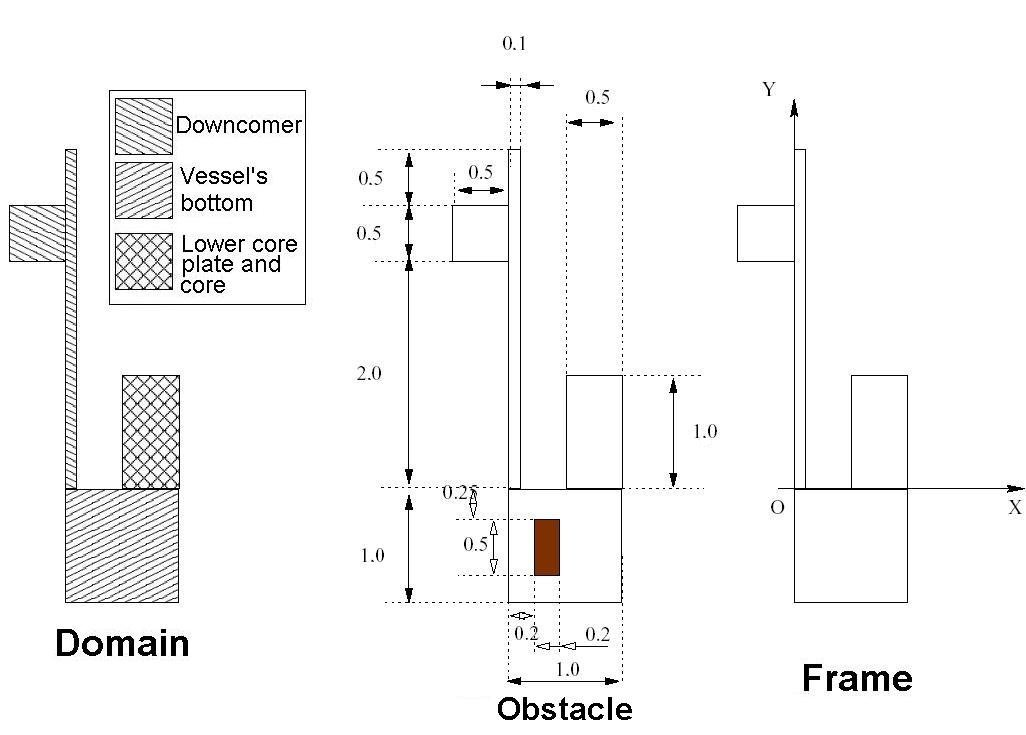
\includegraphics[width=10cm,height=8cm]{fig09}
\caption{Full domain geometry with the obstacle}
\label{figante41}
\end{center}
\end{figure}


        \subsection{Parameters}
%------------------------------

All the parameters necessary to this study can be defined through the Graphical
Interface. However, the calculation of the spatial average is defined by a user routine.


\begin{center}
\begin{tabular}{|l|c|}
\hline
\multicolumn{2}{|c|}{Parameters of calculation control} \\
\hline
Number of iterations & $300$ \\
\hline
Reference time step & $0.05$ \\
\hline
Output period for post-processing files& $2$ \\
\hline
The calculation will be run in parallel on 2 processors \\
\end{tabular}\\
\end{center}

In order to join the separate meshes into a single domain, colors 5, 24 and 32
will have to be joined through the Graphical Interface.


        \subsection{User routines}
%---------------------------------

The following routines have to be copied from the folder SRC/REFERENCE/base into the
folder SRC\footnote{only when they appear in the SRC directory will they be
taken into account by the code}: usclim.f90 and usproj.f90.

$\bullet$ {\bfseries usclim.f90}\\
This routine allows to define advanced boundary conditions on the boundary
faces. Even if usclim.f90 is used, all boundary conditions have to be defined in
the Graphical User Interface. Only the conditions that differ from this first
definition need to appear in usclim.f90. The boundary conditions defined in usclim.f90
will replace those specified in the Graphical Interface.

In this case, the temperature at entry is supposed variable in time, following
the law:
\begin{equation}
\left\{\begin{array}{ll}
T = 20 + 100t & \text{for }0\leqslant t \leqslant 3.8\\
T = 400 & \text{for } t > 3.8
\end{array}\right.
\end{equation}
where $T$ is the temperature in \degresC\ and $t$ is the time in $s$.


\begin{figure}[h!]
\begin{center}
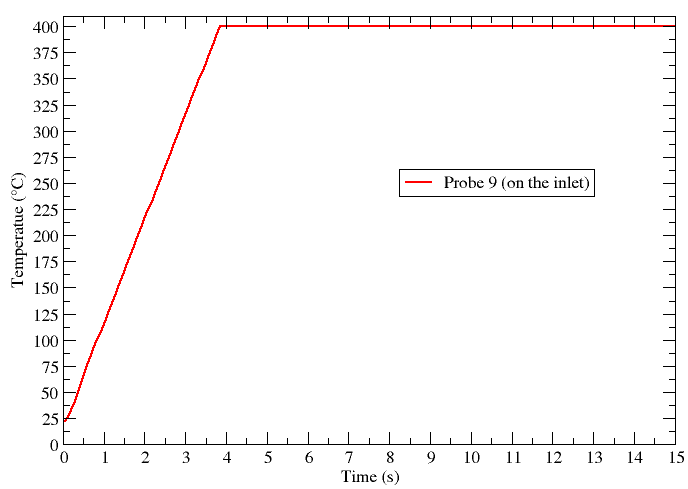
\includegraphics[width=9cm,height=6.4cm]{probe9}
\caption{Time evolution of the temperature at inlet}
\label{figp9_e4}
\end{center}
\end{figure}


$\bullet$ {\bfseries usproj.f90}\\
This routine is called at the end of each time step and has access to the whole
set of variables of the code. It is therefore useful for many user-specific
post-processing, including the calculation of a spatial average in the present
case.\\
The spatial average of the temperature will be calculated at each time step and
the result wrote in a file named ``moy.dat''. The values are saved in order
to draw the time evolution of the average temperature.

Beware when calculating the average. Since the calculation is running in
parallel, computing the sum of the temperatures on ``all the cells'' will only
yield for each processor the sum on the cells managed by this processor. In
order to obtain the full sum, the parallelism routine PARSOM must be used (see
example).

\textbf{Note:} usproj.f90 contains many examples. They should be removed before
running the case.


        \subsection{Output management}
%-------------------------------------

The output management is the same as in case 3.

\begin{figure}[htp]
\parbox{8cm}{%
\centerline{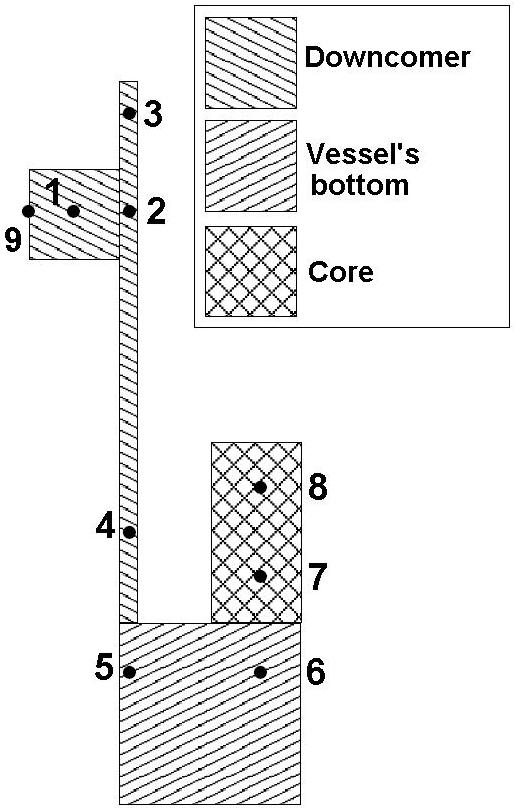
\includegraphics[width=4cm,height=6.8cm]{fig08}}}
\parbox{7cm}{%
\begin{center}
\begin{tabular}{|c|c|c|c|}
\hline
Points & X(m) & Y(m) & Z(m)\\
\hline
1 & -0.25 & 2.25 & 0 \\
\hline
2 & 0.05 & 2.25 & 0 \\
\hline
3 & 0.05 & 2.75 & 0 \\
\hline
4 & 0.05 & 0.5 & 0 \\
\hline
5 & 0.05 & -0.25 & 0 \\
\hline
6 & 0.75 & -0.25 & 0 \\
\hline
7 & 0.75 & 0.25 & 0 \\
\hline
8 & 0.75 & 0.75 & 0 \\
\hline
9 & -0.5 & 2.25 & 0 \\
\hline
\end{tabular}
\end{center}
}
\caption{Position and coordinates of probes in the full domain}
\label{figante42}
\end{figure}

In this case, the {\itshape Pressure}, the {\itshape Tubulent energy} and the
{\itshape Dissipation} will be removed from the listing file.

The {\itshape Courant number} (CFL) and {\itshape Fourier number} will be
removed from the
post-processing results\footnote{this can be very useful to save some disk space
if some variables are of no interest, as post-processing files can be large}.

Eventually, probes will be defined for chronological records, following the data
given in figure \ref{figante25}. Then the {\itshape total pressure} will be
deactivated from all probes and the {\itshape Velocity U} will be only activated
on probes  1, 2, 6, 7 and 8.


In addition the domain boundary will be post-processed. This allows to check the
boundary conditions, and especially that of the temperature and passive scalar.



        \subsection{Results}
%---------------------------
Figure \ref{fige2_e4} shows the evolution of the spatial average of the temperature.

\begin{figure}[h]
\begin{center}
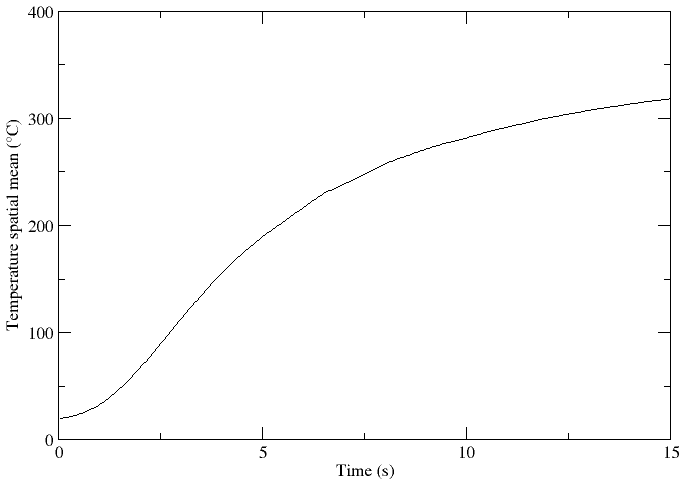
\includegraphics[width=9cm]{moytemp}
\caption{Evolution of spatial average of the temperature as a function of time}
\label{fige2_e4}
\end{center}
\end{figure}

Figure \ref{fige1_e4} shows velocity fields colored by temperature. The effect
of the head loss modeling the obstacle is clearly visible.

\begin{figure}
\begin{center}
\begin{tabular}{cc}
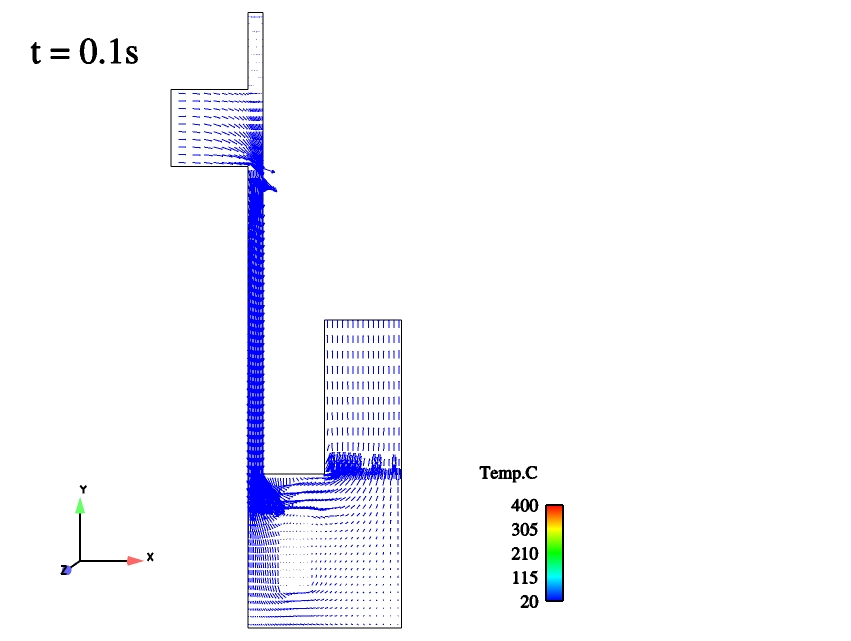
\includegraphics[height=6cm]{case4_p1} &
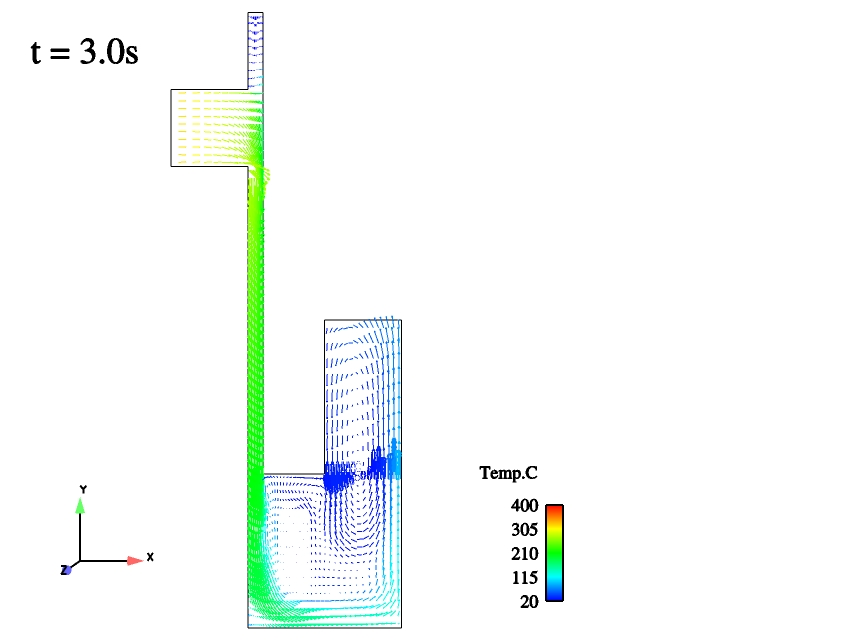
\includegraphics[height=6cm]{case4_p2} \\
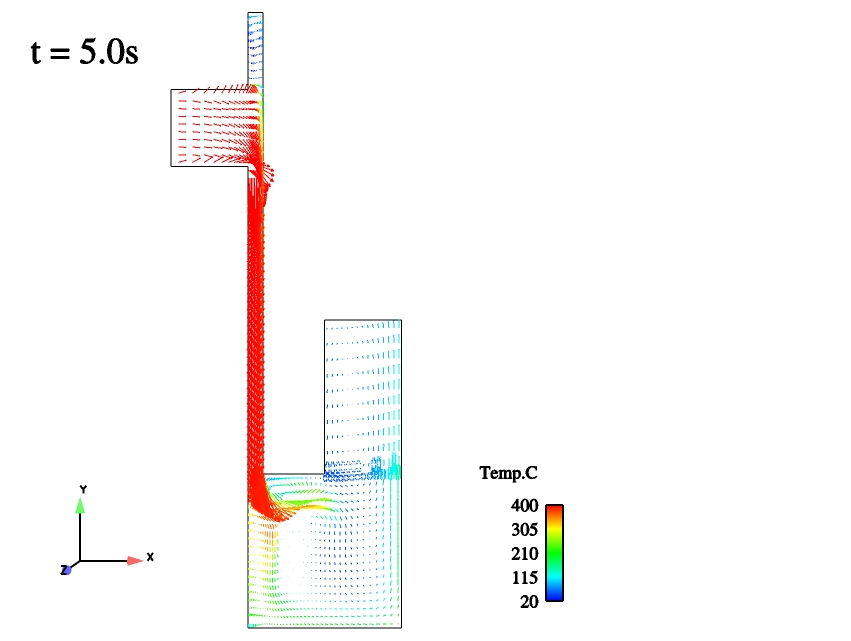
\includegraphics[height=6cm]{case4_p3} &
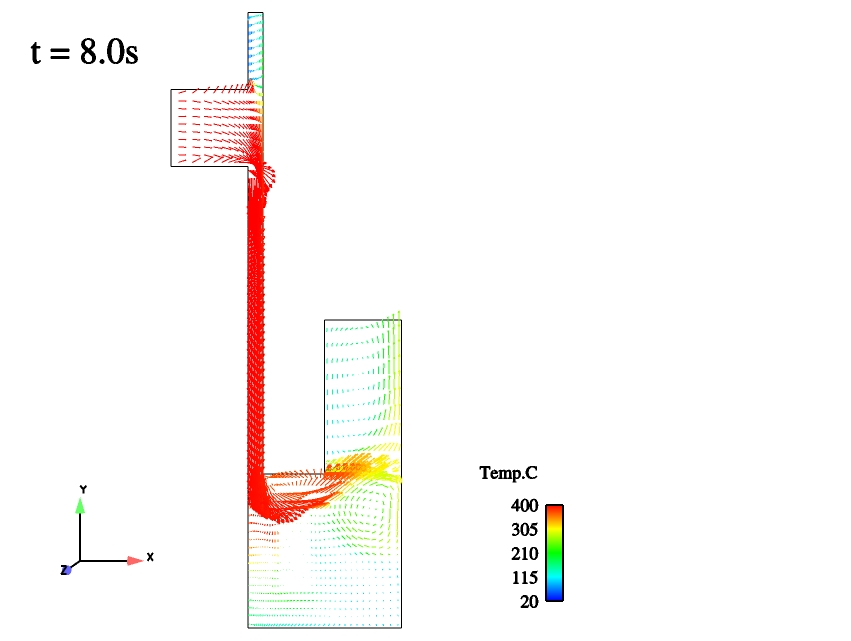
\includegraphics[height=6cm]{case4_p4} \\
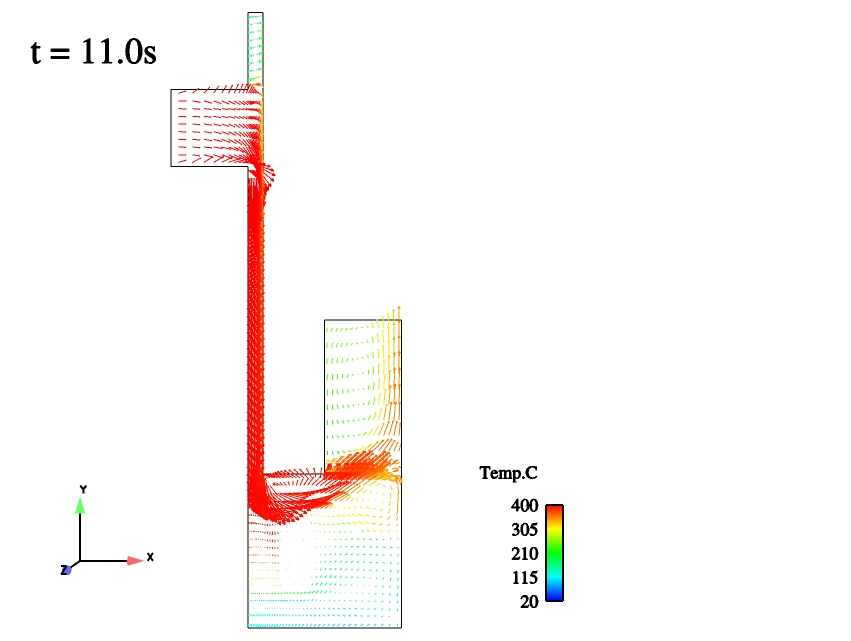
\includegraphics[height=6cm]{case4_p5} &
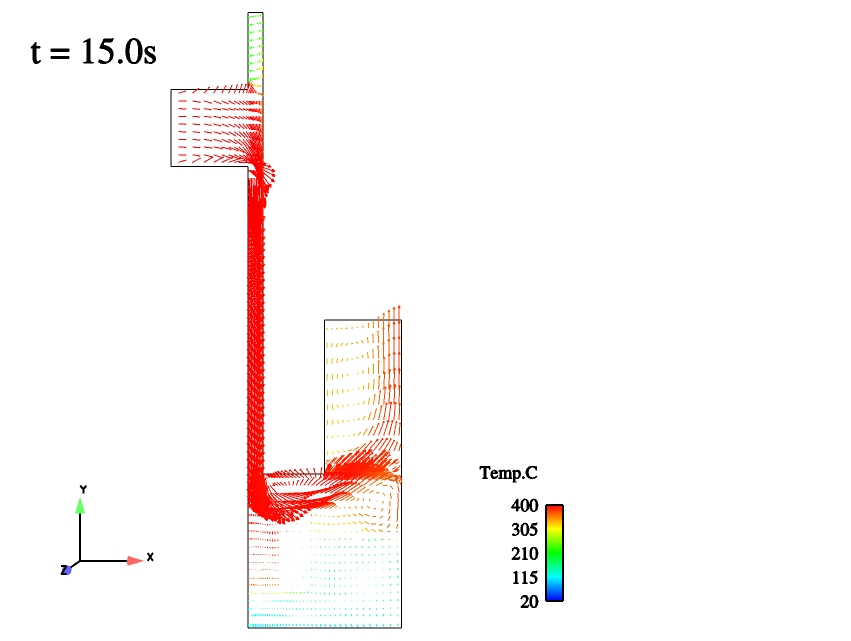
\includegraphics[height=6cm]{case4_p6} \\
\end{tabular}
\caption{Water velocity field colored by temperature}
\label{fige1_e4}
\end{center}
\end{figure}


